%Estado del Arte: Fundamentos teóricos o Marco teorico
\chapter{Estado del Arte}\label{sec:capitulo3}
\thispagestyle{empty}
El presente capítulo establece las bases teóricas de este trabajo, de forma resumida y concisa, con el objetivo de familiarizar al lector con los conceptos necesarios para una efectiva comprensión de los temas a tratar. En este orden de ideas, se introducirán conceptos vinculados con las bases sobre las cuales estan hechas las comunicaciones hoy en día, tanto comerciales como vehículares, y de esta forma poder hablar con más criterio sobre los sistemas de comunicaciones comerciales y vehículares, describiendo los protocolos e instrumentos fundamentales para su funcionamiento.\\

\par Seguidamente, se expone la sección relacionada con los sistemas cooperativos, donde se dará a conocer toda la información de interés referente a estos sistemas, así como de los ADAS, para luego describir distintas maniobas cooperativas que se pueden realizar hoy en día. Por último se mencionará la estrategia de control implementada en la realización de las maniobras, dicha estrategia se basa en la lógica difusa, por lo que primero se procederá a definir la misma, para luego entender su utilización en el área de control.\\  
    
\section{Revisión Bibliográfica}

En esta sección se procederá a hacer un repaso a los campos de investigación relacionados a las redes de comunicación, los cuales serán de ayuda para un mejor entendimiento de los demás temas tratados en este trabajo.

\subsection{Modelo OSI}

Para efectuar una correcta comunicación entre vehículos, infraestructuras o simplemente entre dispositivos comerciales como por ejemplo unos routers, se deben tener ciertas normas que las rijan, es por esto que en esta sección se hará una breve introducción a la división de las normas de comunicación que afectan los distintos sistemas, así como la estructura lógica que deben poseer para que, sin importar las condiciones puedan interactuar entre si.\\

\par Propiamente el modelo de interconexión de sistemas abiertos, modelo OSI (del inglés, \textit{Open System Interconnection}) es una recomendación o normas de comunicaciones que deben de seguir los fabricantes para que todos los dispositivos puedan comunicarse entre ellos independientemente de la tecnología empleada \cite{anaya2016sistema}. Fue creado en el año 1980 por la organización internacional de normalización, ISO (del inglés, \textit{International Organization for Standardization}), siendo publicado oficialmente en el año 1983 por la unión internacional de telecomunicaciones, ITU (del inglés, \textit{International Telecommunications Union}).\\

\par El modelo está conformado por siete capas que definen las diferentes fases por las cuales los datos deben pasar para ir de un dispositivo a otro sobre una red de comunicaciones (ver figura \ref{fig:osi}). Sobre este esquema se han creado numerosos protocolos, los cuales cada vez están siendo más flexibles, reduciendo el número de capas y logrando transiciones de niveles no tan demarcadas, por lo que, el modelo OSI está quedando cada vez más obsoleto al pasar de los años, pero para efectos de los sistemas analizados en este trabajo la norma aún sirve como referente para su entendimiento, dicho esto se procederá a describir cada uno de los niveles.\\

\begin{figure}[hbp]
	\centering
		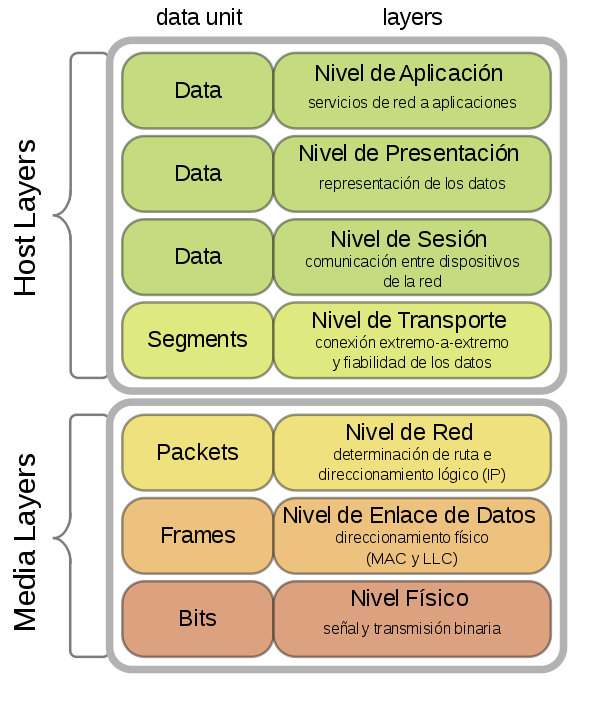
\includegraphics[scale=0.4]{Imagenes/osi}
		\caption{Torre OSI \cite{anaya2016sistema}}
		\label{fig:osi}
	\end{figure}	

\begin{itemize}
	\item Nivel físico: es el primer nivel presentado en el modelo, es el encargado de la topología de red y de las conexiones del dispositivo hacia la msima. Está más enfocado al medio físico y de como se transmite la inoformación en este.
	\item Nivel de enlace de datos: es el nivel encargado: del direccionamiento físico, del acceso al medio, de la distribución ordenada de las tramas y del control del flujo de datos.
	\item Nivel de red: se encarga de identificar el enrutamiento existente entre varias redes, es en este nivel donde se realiza el direccionamiento lógico y se establece la ruta que tienen que seguir los datos del origen hasta el receptor final.
	\item Nivel de transporte: es el encargado de realizar el transporte de los datos del dispositivo origen, al dispositivo destino, esto independientemente del tipo de red física empleada.
	\item Nivel de sesión: es el nivel encargado de mantener y controlar el enlace establecido entre los dispositivos.
	\item Nivel de presentación: en este nivel se traduce la información, de tal forma que distintos dispositivos puedan entender la información que reciben independiente de las diferentes representaciones internas que estos puedan tener.
	\item Nivel de aplicación: es el último nivel del modelo, responsable de ofrecer a las aplicaciones la posibilidad de acceder a los distintos servicios de los demás niveles, así como también definir los protocolos que utilizan estas aplicaciones para intercambiar los datos.
\end{itemize}

\subsection{Redes Ad-Hoc}
Las redes ad hoc, son redes inalámbricas que no requieren de ningún tipo de infraestructura fija ni administración centralizada, donde cada componente es una estación capaz de ofrecer servicios de encaminamiento, retransmitiendo paquetes de otras estaciones que no posean conexión inalámbrica directa. Estas redes son capaces de desplegarse tanto de forma autónoma como de forma combinada con las redes locales, y de esta manera gozar los beneficios de los servicios de internet \cite{orozco2012redes}. Vieron sus comienzos en los años 70, siendo conocidas con el nombre de radio paquetes, nombre que fue cambiado en los años 80 por el de redes ad-hoc, dicho cambio se produjo a raíz de ser implementadas en proyectos militares, los cuales las renombraron como se conoce actualmente(6). En la figura \ref{fig:adhoc} se puede encontrar un ejemplo de la distrubución del internet a través de una red ad-hoc.\\

\begin{figure}[hbp]
	\centering
		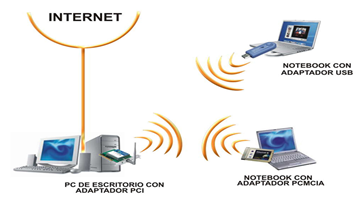
\includegraphics[scale=0.7]{Imagenes/adhoc}
		\caption[Red ad-hoc subordinada a internet]{Red ad-hoc subordinada a internet \protect\footnotemark}
		\label{fig:adhoc}
	\end{figure}	

\footnotetext{http://karolcasierra.blogspot.com/2013/04/red-ad-hoc-movil-caracteristicas-y.html}

\par Dentro de las características más resaltantes se puden encontrar:
\begin{itemize}
	\item Son nodos móviles, es decir los dispositivos de las redes ad-hoc pueden cambiar de posición a placer.
	\item Constan de una topología variable, ya que los dispositivos se pueden mover y formar nuevos elances con otros dispositivos, siempre y cuando pertenezcan a su área de cobertura.
	\item Tienden a realizar cambios de ruta, esto debido a su topología variable, lo cual produce que la ruptura de enlaces sea un problema frecuente, lo que origina que se varien las rutas constantemente.
	\item Poseen autonomía limitada causada por la portabilidad de los dispositivos, ya que estos vienen limitados en cuanto a la duración de la batería.
	\item Tienen limitaciones en los enlaces inalámbricos, ya que estos enlaces se caracterizan por tener un ancho de banda reducido, asi como, una disposición a comerter errores, defectos que se ven compensados por la cualidad de repetidor de nodos. 
	\item Gozan de la ausencia de infraestructura, esto debido a que no existe ningún tipo de entidad centralizada que rijan las conexiones, por lo cual los dispositivos pueden desempeñar los papeles de host o router en cualquier momento.
\end{itemize}

 Según su aplicación se pueden clasificar de la siguiente manera: 
\begin{itemize}
	\item Redes ad-hoc móviles, MANET's (del inglés, \textit{Moblie Ad-Hoc Networks}).
	\item Redes inalámbricas malladas.
	\item Redes de sensores.
	\item Redes ad-hoc vehiculares, VANET's (del inglés, \textit{Vehicular Ad-Hoc Networks}).
\end{itemize}

\subsection{Protocolos de Transporte}

Entre las capas expuestas anteriormete se encuentra la de transporte, pieza fundamental de la arquitectura del modelo. Desempeñando un papel crítico al proporcionar servicios de comunicación a los procesos de aplicación que se ejecutan en hosts diferentes. Dentro de estos protocolos se pueden destacar tres, dos para las comunicaciones entre componentes comerciales, e internet, UDP y TCP, y uno para las comunicaciones vehiculares, \textit{Geonetwork}.

\subsubsection{UDP}

El protocolo de datagrama de usuario, UDP (del inglés, \textit{User Datagram Protocol}) es un protocolo del nivel de transporte basado en el intercambio de datagramas El mismo permite el envío de dichos datagramas a través de la red sin que se haya establecido una conexión previa, esto debido a que los mismos incorporan sufiente información de direccionamiento. Además no posee confirmación ni control de flujo, lo que origina que los paquetes puedan adelantarse unos a otros y se pierdan en el camino. Este tipo de protocolo es mayormente empleado para servidores DHCP, BOOT y DNS, y demás servicios en los que el intercambio de paquetes de la conexión son mayores, o  no son rentables con respecto a la información trnasmitida (3). Entre las principales características se encuentra que:\\

 \begin{itemize}
	\item Es un protocolo mínimo de nivel de transporte orientado a los mensajes.
	\item Proporciona una sencilla interfaz entre la capa de red y la capa de aplicación.
	\item No otorga garantías para la entrega de sus mensajes.
	\item Es empleado cuando resulta más importante transmitir con velocidad que garantizar el hecho de que los mensajes lleguen completos, como es el caso de la transmisión de audio y video.
\end{itemize}

\subsubsection{TCP}
El protocolo de control de transmisión, TCP (del inglés, \textit{Transmission Control Protocol}) es un protocolo orientado para crear conexiones entre computadoras de una misma red. En este caso el protocolo garantiza que los datos serán entregados a su destino sin errores y en el mismo orden en el cual fueron transmitidos. TCP da soporte a muchas aplicaciones relacionadas al internet, como lo pueden ser: navegadores, intercambio de ficheros, proramas de mensajería entre otros (3). Entre las principales características se ecnuentra que: 

\begin{itemize}
	\item Es orientado a la conexión, es decir las computadoras se conectan para intercambiar datos, sincronizandose para manejar el flujo de paquetes y adaptarse a la congestión de red.
	\item Emplea la técnica cheksum, con la cual verifica que los paquetes no esten corruptos.
	\item El receptor regresa un acuse de recibo al transmisor indicando que ya llegaron los paquetes.
	\item En caso de se desborde el buffer receptor, el mismo descarta los paquetes, ocasionando que el transmisor reduzca la tasa de envío.
	\item En caso de que el mensaje no se reciva de forma adecuada e receptor puede pedir la retransmisión del mismo.
\end{itemize}

\section{Sistemas de Comunicación}

A continuación se presentan los fundamentos sobre los sistemas de comunicación analizados en este trabajo.\\ 

\subsection{Sistemas de Comunicación Comerciales}
Los sistemas de comunicación comerciales son aquellos elementos empleados para conectar distintos dispositivos, ya sean computadoras, celulares, televisores, etc. Son nombrado como comerciales, ya que son de acceso al público sin ninguna restricción. Estos sistemas hacen uso de los dispositivos de comunicación como lo son los routers, o enrutadores y los puntos de acceso, AP (del inglés, \textit{Access Point}) \cite{pellejero2006fundamentos}.\\

 \begin{itemize}
	\item Router: es un dispositivo que porporciona conectividad a nivel de red, o nivel tres del modelo OSI, cuyo principal objetivo consiste en enviar o encaminar paquetes de datos de una red a otra, es decir interconectar subredes (Figura \ref{fig:router}).

\begin{figure}[!h]
	\centering
		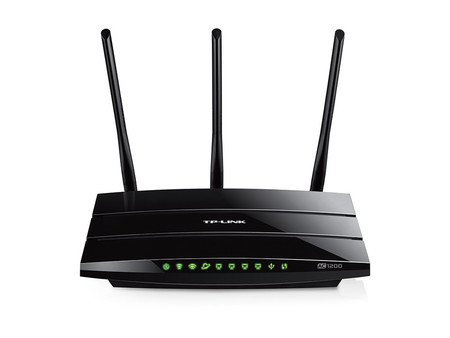
\includegraphics[scale=0.5]{Imagenes/router}
		\caption{Ejemplo de un router}
		\label{fig:router}
	\end{figure}	

	\item Punto de Acceso: es un dispositivo de red que interconecta equipos de comunicaciones inalámbricos, para formar una red, en la cual se conectan distintos elementos móviles o trajetas de red inalámbricas (Figura \ref{fig:pa}).

\begin{figure}[!h]
	\centering
		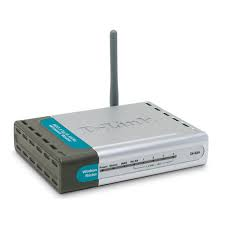
\includegraphics[scale=0.5]{Imagenes/pa}
		\caption{Ejemplo de un punto de acceso}
		\label{fig:pa}
	\end{figure}	
\end{itemize}   

\subsubsection{W-Lan}

Las redes WLAN (Figura \ref{fig:wlan}). se pueden definir como un sistema de comunicación que transmite y recibe datos utilizando ondas electromagnéticas, en vez de un cable trenzado o fibra óptica utilizado en las LAN, y que proporciona conectividad inlámbrica, dentro de un área de cobertura determinado, entre 10 m y 100 m\cite{varela2002redes}. Dentro de sus características más importantes se encuentran:\\

\begin{figure}[!h]
	\centering
		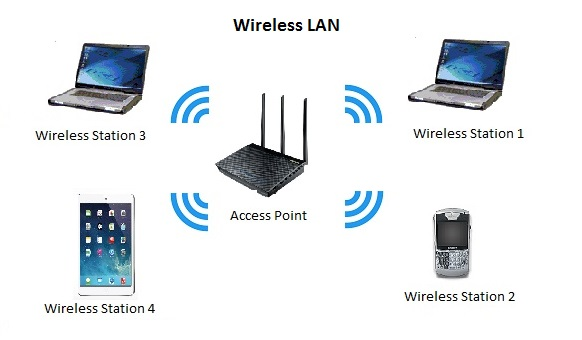
\includegraphics[scale=0.6]{Imagenes/wlan}
		\caption[Ejemplo de una WLAN, for L0F]{Ejemplo de una WLAN \protect\footnotemark}
		\label{fig:wlan}
	\end{figure}	
\footnotetext{http://tiposderedesgeograficamente.blogspot.com/}

\begin{itemize}
	\item Movilidad: permite transmitir información en tiempo real en cualquier lugar de la organización o empresa a cualquier usuario.
	\item Facilidad de instalación: al no usar cables, se evitan arduos trabajos de instalación de los mismos, por lo que se reduce el tiempo neceseario para poder emplear los servicios de red, además de proporcionar los servicios a múltiples usuarios de forma instantánea.
	\item Flexibilidad: puede llegar a donde no puede el cable, aumentando así el rango de cobertura. Además de ser más económica que los sistemas cableados.
\end{itemize}

Las WLAN poseen un gran número de escenarios en los cuales pueden ser empleados, siendo los mas destacados destacados:\\

\begin{itemize}
	\item Escenario residencial: una línea telefónica terminada en un router ADSL al cual se conecta un punto de acceso, para formar una red WLAN que de cobertura a varios dispositivos.
	\item Redes corporativas: una serie de puntos de accesos distruibuidos en varias áreas de la empresa que conforman redes autonómas.
	\item Acceso a internet desde distintos lugares: desde cafeterías hasta medios de transportes que poseen conexión via satelital, los cuales pueden proporcionar servicios de internet a los usarios conectados a su red.
	\item Usos corporativos e industriales: como interconexiones de máquinas y distintos dispositivos.   
\end{itemize}

\par Otro uso que, tomando en cuenta sus específicas condiciones no es tán común, como pueden ser cualquiera de los mencionados, es el uso en comunicaciones vehiculares, esto debido a que son conexiones con características muy particulares que una simple red WLAN no puede garantizar cumplir, a excepción de algunos casos, donde bajo ciertas condiciones se puede recrear este tipo de comunciaciones, como se va a mostrar más adelante en los siguientes capítulos.\\    

\par Las WLAN emplean principalmente las bandas industriales, científicas y médicas, ISM (del inglés, \textit{Industrial, Scientific and Medical}), que comprenden las frecuencias entre 902-928 MHz, 2.4-2.4835 GHz y 5.725-5.850 GHz. Estas bandas son de uso común y no requieren de licencia para utilizarlas. Debido a que estas frecuencias no requieren de licencia para operar las WLAN poseen un gran potencial de mercado logrando así competir con otros tipos de tecnologías de acceso, lo cual obliga que se desarrolle un marco regulatorio que permita el uso eficiente y compartido de las mismas. En este ámbito es donde entra el instituto de ingenieros eléctricos y electrónicos, IEEE (del inglés, \textit{Institute of Electical and Electronic Engineers}), el cual dasarrolló los estándares que rigen este tipo de red, estándares que se procederán a describir a continuación.

\subsubsection{IEE 802.11}  

Las redes WLAN cumplen con los estándares genéricos aplicables al mundo de las LAN cableadas, pero necesitan una normativa adicional que defina el uso y acceso de los recursos radioeléctricos. Estas normativas definen de forma detallada los protocolos para las capas física, de control de acceso al medio, MAC (del inglés, \textit{Media Acces Control}) y de control de enlace de datos, DLC (del inglés, \textit{Data Link Level}) que regulan la conexión vía radio\cite{camargo2009modelo}. El primer estándar donde se especificaron estas capas fue el IEEE 802.11 en el año 1997.\\

\par Este estándar especifica una frecuencia de operación de 2.4 GHz con velocidades de transmisión de 1 y 2 Mbps. Desde esta versón inicial el IEEE 802.11 WG (del inglés, \textit{Working Group}) ha llevado a cabo diferentes revisiones a través de varios grupos de trabajo especializados en distintas áreas.\\

 \par Antes de repasar cada uno de estos estándares se procederá a describir el esquema de las capas (Figura \ref{fig:ieee}), que es común para cada uno ellos.\\ 

\begin{figure}[H]
	\centering
		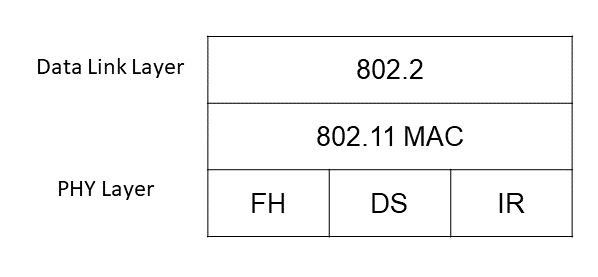
\includegraphics[scale=0.5]{Imagenes/ieee}
		\caption{Capas del IEEE 802.11 \cite{{pellejero2006fundamentos}}}
		\label{fig:ieee}
	\end{figure}	

\par Donde:

 \begin{itemize}
	\item La Capa física: define la modulación y la señalización característica de la transmisión de datos. Como se mencionó anteriormente estas redes operan en la banda de 2.4 GHz a excepción del IEEE 802.11 a que opera en la banda de 5 GHz, ocupando aproximadamente 83 MHz de ancho de banda. Para la transmisión y recepción de tramas se tienen tres opciones:
	\begin{itemize}
		\item Espectro expandido por secuencia diercta, DSS (del inglés, \textit{Direct Sequence Spread Spectrum})
		\item Espectro expandido por salto de frecuencia, FHSS (del inglés, \textit{ Frequency Hopping Spread Spectrum})
		\item Modulación por división ortogonal de frecuencias, OFDM (del inglés, \textit{Orthogonal Frequency Division 					Multiplexing})
	\end{itemize}	
	\item Capa MAC: es la capa de control del medio, para la cual se diseñó un mecanismo que puede reaccionar positivamente ante 		perturbaciones ambientales, variaciones en la potencia de la señal, y las repentinas conexiones y desconexioes en la red. Este 		mecanismo es conocido como, acceso múltiple por detección de portadora y prevención de colisiones, CSMA/CA (del inglés, \textit{Carrier Sense Multiple Acces with Collision Avoidance}), que funciona de la siguiente forma, si la estación que desea 			transmitir escucha el medio de transmisión, pero si el medio esta ocupado significa que otra estación está transmitiendo y por lo 		tanto debe de retrasar su transmisión hasta que se libere.
\end{itemize}

\par Ya conociendo la estructura básica de del IEEE 802.11 ahora se procede a hablar sobre cada uno de los estándares \cite{pellejero2006fundamentos}.

 \begin{itemize}
\item 802.11a: es un estándar también conocido como Wi-Fi5. Su misión es crear un estándar de WLAN en la banda de 5 GHz, capaz de alcanzar tasas de hasta 54 Mbps. Se publicó en el 1999.
\item  802.11b: es un estándar también conocido como Wi-Fi. Está pensado para WLAN en la banda de 2.4 GHz, con una tasa que alcanza los 11 Mbps. Fue publicada en el 1999.
\item  802.11c: provee de documentación a la 802.11 sobre procedimientos específicos MAC de la Organización Internacional para la Comisión Electrónica de Estandarización Internacional (ISO/IEC). Su trabajo está concluido.
\item  802.11d: su misión es definir nuevos requerimientos para la capa física para hacer funcionar la 802.11 en otros países donde no es posible implementar 802.11, por no tener la banda de 2.4 GHz libre o ser más corta.
\item  802.11e: este grupo trabaja en los aspectos relacionados con la calidad de servicio, QoS (del inglés, \textit{Quality of Service}). En el mundo de las redes de datos, calidad de servicio significa poder dar más prioridad de transmisión a unos paquetes de datos que a otros, dependiendo de la naturaleza de la información (voz, vídeo, imágenes, etc.).
\item  802.11f: básicamente, es una especificación que funciona bajo el estándar 802.11g y que se aplica a la intercomunicación entre puntos de acceso de distintos fabricantes, permitiendo el roaming o itinerancia de clientes.
\item  802.11g: pretende desarrollar una extensión de la 802.11b, \textit{higherspeed PHY}, capaz de mantener la compatibilidad con la 802.11b. El objetivo inicial de este era alcanzar al menos 20 Mbps y se ha conseguido llegar hasta los 54 Mbps.
\item  802.11h: una evolución del IEEE 802.11a que permite asignación dinámica de canales y control automático de potencia para minimizar los efectos de posibles interferencias. Este punto es una de las desventajas que tiene IEEE 802.11a frente a su competidor europeo HiperLAN/2 (que también opera en la banda de los 5 GHz).
\item 802.11i: este estándar permite incorporar mecanismos de seguridad para redes inalámbricas, ofrece una solución interoperable y un patrón robusto para asegurar datos. Mejora los mecanismos de autenticación y seguridad de la 802.11, como es WEP. El sistema sobre el que se está trabajando se conoce como TKIP (del inglés, \textit{Temporal Key Integrity Protocol}).
\item 802.1x: pretende mejorar los mecanismos de seguridad de la 802.11, con los protocolos de seguridad extendida, EAP (del inglés, \textit{Extensible Authentiticatiion Protocol}).
\end{itemize}

\subsection{Sistemas de Comunicación Vehicular}

Los sistemas de comunicación vehicular son los sistemas empleados para la conexión entre vehículos, infraestructuras y peatones, están compuestos básicamente de dos componentes, las unidades a bordo, OBU's (del inglés, \textit{On Board Untis}) y las unidades en vía, RSU's (del inglés, \textit{ Road Side Unit's}) (Figura \ref{fig:obursu}), las cuales tienen como finalidad dar soporte a las comunicaciones de las aplicaciones de diversas naturalezas. La principal diferencia entre ambas, es el propósito por el cual fueron diseñadas. Las OBU's están destinadas a los vehículos, por lo cual pueden cambiar su posición, mientras que las RSU's se encuentran en las infraestructuras, lo que implica que son estáticas.\\

\begin{figure}[!h]
	\centering
		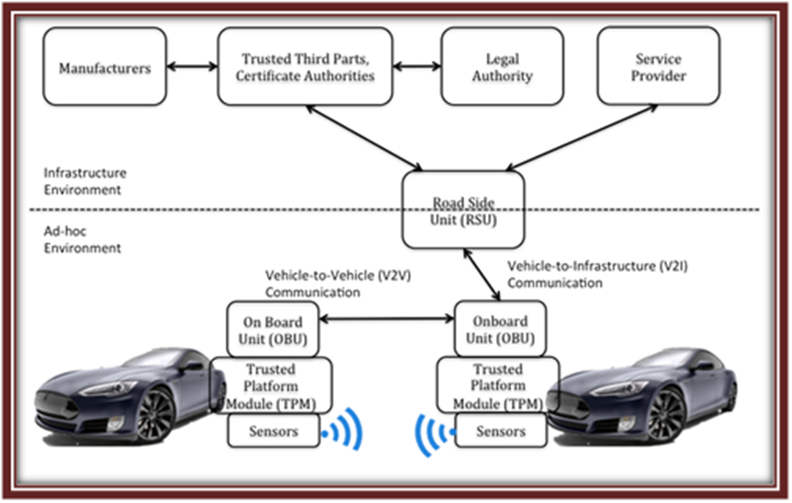
\includegraphics[scale=0.8]{Imagenes/obursu}
		\caption[Ejemplo de la comunicación entre las OBU's y las RSU's, for L0F]{Ejemplo de la comunicación entre las OBU's y las RSU's \protect\footnotemark}
		\label{fig:obursu}
	\end{figure}	
\footnotetext{https://www.cse.wustl.edu/\~jain/cse571-14/ftp/vanet\_security/index.html}

 \par El objetivo de estos sistemas es comunicar los distintos componentes que conforman los ITS, es por eso que se clasifican en cinco tipos\cite{da2014data} (Figura \ref{fig:v2x}):

\begin{itemize}
	\item Vehículo con vehículo, V2V (del inglés, \textit{Vehícle to Vehícle}): es el tipo de comunicación entre vehículos, la cual no necesita de una infraestructura fija que maneje la interacción entre los mismos, es usada por lo general en aplicaciones de seguridad, prevención de riesgos y para esparcir información. Debido a su natruraleza móvil este es un tipo de red ad-hoc vehícular, mejor conocida como VANET's.
	\item Vehículo con infraestructura, V2I (del inglés, \textit{Vehicle to Infrastructure}): es el tipo de comunicación entre vehículos e infraestructura, es usada para esparcir información, así como para recolección de data.
	\item Vehículo con peatón, V2P (del inglés, \textit{Vehicle to Pedestrian}): es el tipo de comunicación entre vehículos y peatones, que en este caso engloba tanto personas que se movilizan a pie, como en bicicleta. En general se utiliza en aplicaciones de prevención de riesgo, así como para la obtención de los servicios de internet por parte de los peatones.
	\item Arquitectura híbrida, V2X (del inglés, \textit{Vehicle to Everething}): es la combinación entre los escenarios planteados anteriormente, V2V, V2I, V2N y V2P. En este caso los vehículos intercambian información con las infrastructuras de forma multi salto o de un solo salto, dependiendo de las distancias.
	\item Vehículo con la red, V2N (del inglés, \textit{Vehicle to Network}): es el tipo de conexión entre los automóviles y los servidores de aplicaciones, el cual tiene como principal función dotar a los carros con los servicios de internet.
\end{itemize}

\begin{figure}[!h]
	\centering
		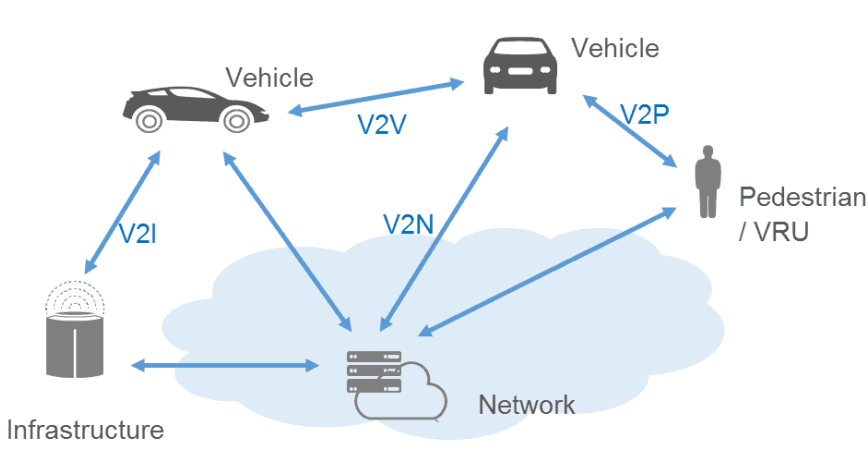
\includegraphics[scale=0.4]{Imagenes/v2x}
		\caption[Tipos de comunicaciones vehículares, for L0F]{Tipos de comunicaciones vehículares \protect\footnotemark}
		\label{fig:v2x}
	\end{figure}	
\footnotetext{http://www.traffictechnologytoday.com/news.php?NewsID=82371}

\subsubsection{Vanets}
El uso de las diversas tecnologías inalámbricas enfocadas a vehículos ha sido objeto de estudio desde los años 70, teniendo como uno de los proyectos pioneros el desarrollado por el ministerio de industria y comercio internacional de Japón, MITTI (del inglés, \textit{Ministry of International Trade and Industry}), que consistió en un sistema integral automovilístico de control de tráfico, CACS (del inglés, \textit{Comprehensive Automovile Traffic Control System}), cuyo objetivo fue reducir la congestión vehicular y disminuir el número de accidentes de tráfico, aportando a los conductores información sobre las vías y asistencia en caso de emergencias \cite{orozco2012redes}.\\

\par En 1986, el proyecto PROMETHEUS (del inglés, \textit{PROgraMme for Euripean Traffic withc Highest Efficiency and Unprecedented Safety}) conformada por 19 países de Europa, impulsó la investigación en comunicaciones móviles inalámbricas con la propuesta Prometheus SR-MRN (del inglés, \textit{Short-Range Mobile Radio Network}), y de esta forma sentó un precedente en el desarrollo de sistemas de conducción vehicular automatizados \cite{heistert}.\\

\par En la década de los 90 \cite{zeadally2012vehicular} surgieron varios proyectos como, PATH (del inglés, \textit{California Partners for Advanced Traffic and Higways}), ASV (del inglés, \textit{Advanced Safety Vehicle}) y PROMOTE CHAUFFEUR, que desarrollaron distintas áreas de la comunicación vehicular, tales como: estándares, arquitectura y diseño de la red, protocolos de enrutamiento, creación de aplicaciones y mejora en los aspectos de seguridad. Dichos progresos conllevaron que el concepto de VANET tomara relevancia en la comunidad científica,  produciendo de esta forma que se realizaran cada vez más proyectos buscando la optimización de este tipo de red. En la figura \ref{fig:vaneth} se pueden encontrar los distintos proyectos realizados desde su comienzos hasta el año 2010.\\

\begin{figure}[!h]
	\centering
		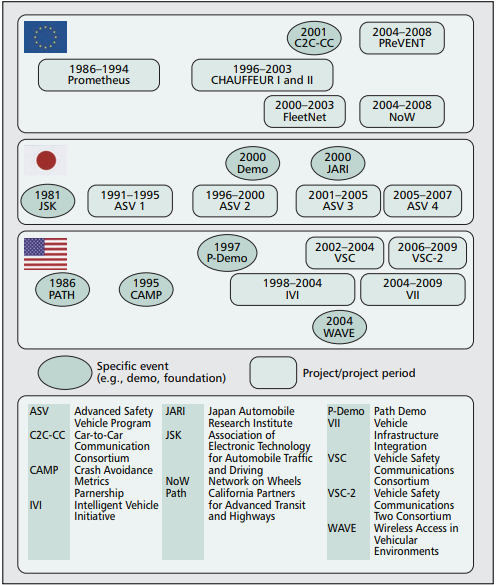
\includegraphics[scale=0.9]{Imagenes/vaneth1}
		\caption{Proyectos relacionados a las VANETS a lo largo de la historia \cite{hartenstein2008tutorial}}
		\label{fig:vaneth}
	\end{figure}	

\par De esta forma se puede decir que las VANET's son una derivación de las redes ad-hoc, donde cada vehículo se define como un nodo de la red capaz de intercambiar información con otros vehículos o con puntos de acceso estacionarios ubicados en las vías.\\

\par Al ser un derivado de las redes ad-hoc, las VANET's poseen las mismas características que estas, con la diferencia, que en este caso los nodos al ser vehículos varian su posición de forma más rápida, lo que produce desconexiones más frecuentes, ocasionando que el intercambio de datos se tenga que realizar de forma muy rápida, y sea propenso a sufrir interferencias de otros enlaces. Debido a estos inconveninetes este tipo de red se diseñó con la intención de que los mismos se afectaran lo menos posbile, así pues distintos entes realizaron sus propias especificaciones, pudiéndose resaltar tres: el ETSI, en Europa, la Comisión Federal de Comunicaciones de Estados Unidos, FCC (del inglés, \textit{Federal Communications Commision}) y la Asociación de Industrias y Negocios de Radio, ARIB, (del inglés, \textit{Association of Radio Industries and Businesses}) \cite{zeadally2012vehicular}. Estas especificaciones se pueden encontrar en la tabla \ref{tab:vanl}.\\

% Table generated by Excel2LaTeX from sheet 'Hoja1'
\begin{table}[htbp]
  \centering
\resizebox{\textwidth}{!}{
    \begin{tabular}{|c|p{14.07em}|p{16em}|c|}
    \toprule
    Característica & \multicolumn{1}{c|}{Japón} & \multicolumn{1}{c|}{Europa} & USA \\
    \midrule
    Tipo de comunicación & Half-duplex (OBU)/Full-duplex(RSU) \& Half-duplex & \multicolumn{1}{c|}{Half-duplex} & Half-duplex \\
    \midrule
    \multicolumn{1}{|p{8.715em}|}{Banda y radiofrecuencia} & Ubicado en la banda de 5.8 GHz, con un ancho de banda de 80 MHz \& Ubicado en la banda de 5.9 GHz & Ubicado en la banda de 5.9 GHz, con un ancho de banda de 20 MHz & \multicolumn{1}{p{12.57em}|}{Ubicado en la banda de 5.9 GHz,con un ancho de banda de 75 MHz} \\
    \midrule
    Canales & \multicolumn{1}{c|}{30 metros} & \multicolumn{1}{c|}{De 15 a 20 metros} & 1000 metros \\
    \midrule
    Tipo de modulación & 2-ASK, 4-PSK (ASK: modulación por desplazamiento de amplitud, del inglés, \textit{Amplitud-Shift Keying}, PSK: modulación por desplazamiento de fase, del inglés, \textit{Phase Shift Keying}) & OFDM & OFDM \\
    \bottomrule
    \end{tabular}}%
\caption{Comparativa de las especificaciones de las VANET's}
  \label{tab:vanl}%
\end{table}%

\par Para este trabajo las normas a considerar son las realizadas en Europa, ya que, el proyecto fue realizado en España, país que se rije bajo esta normativa.       

\subsubsection{DSRC}

Las comunicaciones de corto alcance, DSRC (del inglés, \textit{ Dedicated Short Range Communication}) son comunicaciones inalámbricas bidireccionales, de medio a corto alcance, que permiten una transmición de data a alta velocidad, lo cual es una cualidad muy importante a la de hora enviar los mensajes de seguridad y de las aplicaciones preventivas. Debido a su estructuración, la misma está diseñada específicamente para el uso en comunicaciones V2V y V2I. En Europa las DSRC están diseñadas bajo la arquitectura de acceso a comunicaciones terrestres móviles, CALM (del inglés, \textit{Communications Acces for Land Mobiles}) (Figura \ref{fig:calm}), las cuales están basadas en el modelo de capas OSI.\\

\begin{figure}[!h]
	\centering
		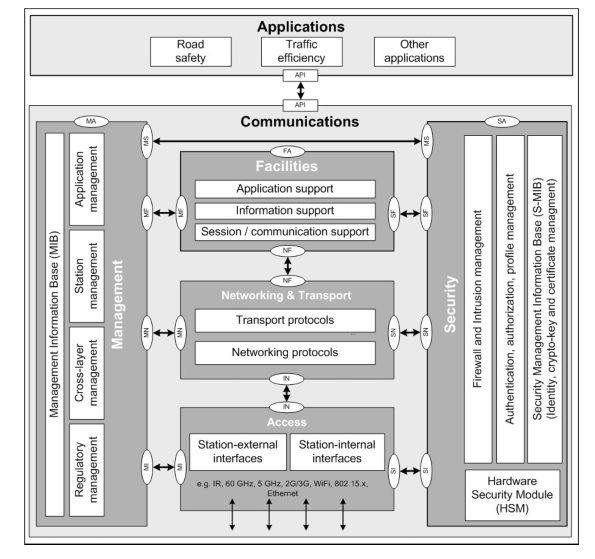
\includegraphics[scale=0.9]{Imagenes/calm}
		\caption{Arquitectura CALM \cite{anaya2016sistema}}
		\label{fig:calm}
	\end{figure}	

\par Esta arquitectura además de ser diseñada por el ETSI, también fue creada por varios entes europeos como lo son: la organización europea de estandarización, ESO's (del inglés, \textit{European Standardization Organizations}) y el comité europeo de estandarización, CEN (del inglés, \textit{European Committee for Standardization}). Unidos, realizaron la ISO/TC204WG16, que es un conjunto de documentos donde se detalla toda la información referente a las DSRC. En la Figura \ref{fig:layers} se puede observar una distribución de la arquitectura CALM, un poco más detallada, indicando las capas con sus respectivos contenidos y los documentos donde se hablan de las mismas \cite{festag2014cooperative}.\\

\begin{figure}[!h]
	\centering
		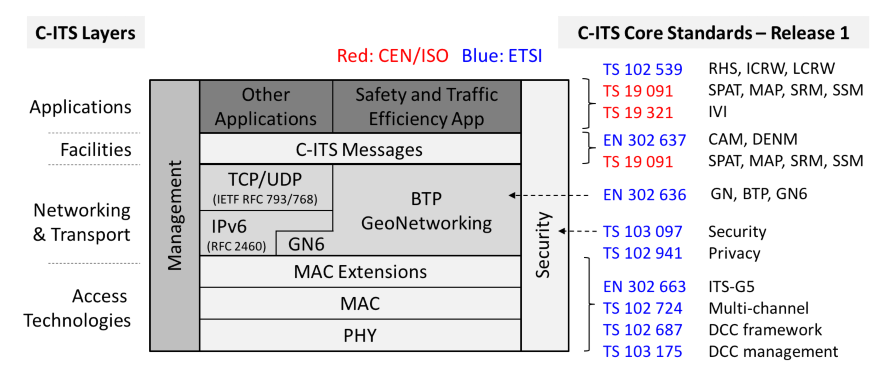
\includegraphics[scale=0.7]{Imagenes/layers}
		\caption{Capas de la arquitectura CALM, con los respectivos documentos donde se encuentran \cite{festag2014cooperative}}
		\label{fig:layers}
	\end{figure}	

\par Entonces, cada capa posee las siguientes especificaciones:

\begin{itemize}
	\item Capa de acceso: está basada en el estándar IEEE 802.11p, donde se poseen tres bandas de frecuencia de 5 GHz, distruibuidas como se muestra en la Figura \ref{fig:fisi}, donde los dos primeros canales se emplean para aplicaciones cualquieras, dejando los otros 5 para ellas aplicaciones de segurdad. Dichos canales de poseen un ancho de 20 MHz, mientras que los demás de 10 MHz. En esta capa se tienen dos niveles: el nivel físico y de MAC, siendo los equivalentes a los niveles 1 y 2 del modelo OSI.\\

\begin{figure}[!h]
	\centering
		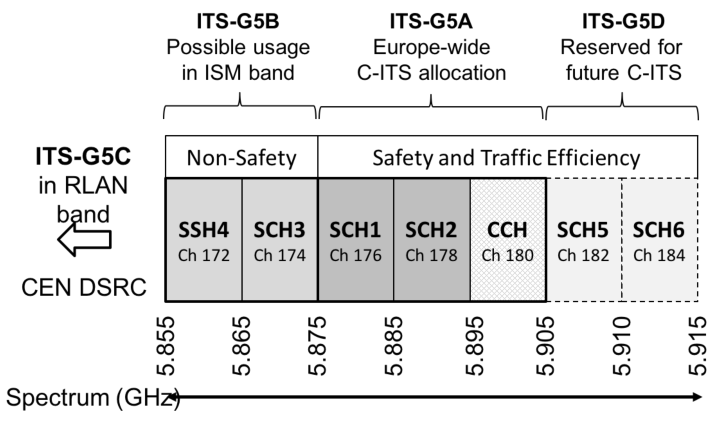
\includegraphics[scale=0.7]{Imagenes/fisi}
		\caption{Distribución de canales en la capa de acceso \cite{festag2014cooperative}}
		\label{fig:fisi}
	\end{figure}	

	\subitem Nivel físico: es en donde se da la transmisión física, la cual emplea, al igual que el estándar IEEE 802.11a una OFDM con 52 subportadoras, de las cuales 48 son para data, las mismas poseen una separación de 10 MHz, con una duración de símbolos de 8 ms, que deja un retardo de 1.6 ms para rangos de comunicaciones menores a 1 km. Los enlaces se producen obviando los procedimientos de negociación, como el escaneo del canal, la autenticación y asociación, lo que genera que se produzcan conexiones más rápidas y directas, reduciendo así, el retraso por control de paquetes. Este tipo de enlace es conocido como esquema de encriptación autenticada, OCB (del inglés, \textit{ Offset Codebook Mode}).
	\subitem Nivel MAC: en este nivel se introduce el mismo esquema especificado en los estándares IEE 802.11, el CSMA/CA, optando por el servicio de calidad conocido como EDCA (del inglés, \textit{Enhanced Distributed Channel Access}), el cual asigna prioridades a los canales, dependiendo de ciertos parámetros y condiciones, basados en la clase del tráfico, es decir, si son mensajes de rutina o de eventualidades. Además de estas características, la capa MAC también cuenta con: un \textit{"gatekeeper"}  y un operador multi canal, MCO (del inglés, \textit{Multi-Channel Operator}), donde el \textit{gatekeeper} asegura que las capas superiores puedan transmitir los paquetes dentro de los límites estabecidos por las prioridades y el MCO controla los transceptores para cambair de canales según se necesite.
	\item Capa de red y transporte: es donde se lleva a cabo el transporte de los mensajes, está compuesta por dos protocolo de enrutamiento, \textit{Geonetworking}, e IPv6. Esta capa corresponde a las capas 3 y 4 del modelo OSI.
	\subitem \textit{Geonetworking}: es un protocolo de enrutamiento que provee el transporte de paquetes en una red ad-hoc sin necesidad de una infraestructura que coordine las conexiones. Emplea la posición geográfica para asignar las direcciones a cada vehículo conectado a la red y de esta forma identificarlos,  pudiendo así, efectuar una comunicación eficiente. Para poder realizar esta identificación se envía un paquete a cada nodo en un área determinada descrita por alguna figura geométrica. En conjunto \textit{Geonetworking} maneja cinco formas de envío de paquetes, \textit{geo-unicast},  \textit{geo-broadcast},  \textit{geo-anycast}, \textit{single-hop broadcast} y \textit{topologically-scoped broadcast}, siendo las dos últimas, formas sin direccionamiento geográfico. En el caso del \textit{geo-broadcast} los paquetes son usados para la distribución de mensajes de eventos relacionados al conductor, mientras que los mensajes periódicos de estatus del vehículo son enviados empleando el \textit{single-hop broadcast}.
	\subitem En la pate superior se encuentra las BTP, las cuales permiten un transporte de paquetes similar al de UDP, entre esta capa y la de servicios, además de permitir la transmisión de paquetes de paquetes IPv6 sin modificaciones, cumpliendo con los requisitos de las conexiones vehiculares.  
	\subitem IPv6: es el protocolo de internet empleado para las conexiones con las estructuras de IP fija y celulares. Para poder realizar esta conexión utiliza los protocolos de UDP, TCP. 
	\item Capa de servicios: es en esta capa donde se clasifican los mensajes recibidos y envíados. Basicamente los mensajes se pueden agrupar en dos tipos, los CAM (del inglés, \textit{Cooperative Awareness Message}) y los DENM, (del inglés, \textit{Decentralized Environmental Notification Message}). Esta capa corresponde a las capas  5 y 6 del modelo OSI. 
	\subitem CAM: son mensajes periódicos que proveen la información de estatus del vehículo a los demás ITS cercanos. Su transmisión se activa cuando el conductor se encuentra en una situación segura. Este tipo de mensajes esta compuesto por una cabezera que contiene la información del tipo de mensaje y dirección del transmisor. En pro de reducir el tamaño de estos mensajes, el contenido siguiente a la cabezera varia según la frecuencia en la cual son enviados, es decir los mensajes de alta frecuencia contienen la data dinámica como lo puede ser posición, velocidad, aceleración, etc, mientras que los de frecuencia baja contienen información del rol del vehículo. El período de envío de estos mensajes depende las reglas impuestas por los productores de los módulos de comunicación, siendo el mínimo tiempo permitido 100 ms, y el máximo 1 s.
	\subitem DENM: son mensajes de advertencia, que se generan cuando ocurre un evento no común, como lo puede ser un accidente de tráfico, una falla en los vehículos, etc. A diferencia de los CAM estos mensajes se transmiten en una área determinada, siendo retransmitidos a su vez para poder alcanzar la mayor cobertura posible. Los DENM están compuestos por una cabezera que contiene el tipo del evento, tiempo en que se detectó, posición etc. seguidamente del cuerpo, donde se da la completa descripción del evento. Estos mensajes son transmitidos a bajas frecuencias, inferiores a la de los CAM. 
	\item Capa de aplicaciones: Es la capa final, donde se clasifican las aplicaciones a las que estan destinados los mensajes. Básicamente la aplicaciones son cuatro: Seguridad vial, servicios locales, servicios de internet y eficiencia del tráfico. Esta capa corresponde a la séptima y última capa del modelo OSI.
\end{itemize}



\section{Sistemas Cooperativos}



\begin{wrapfigure}{r}{10cm}
	\begin{center}
		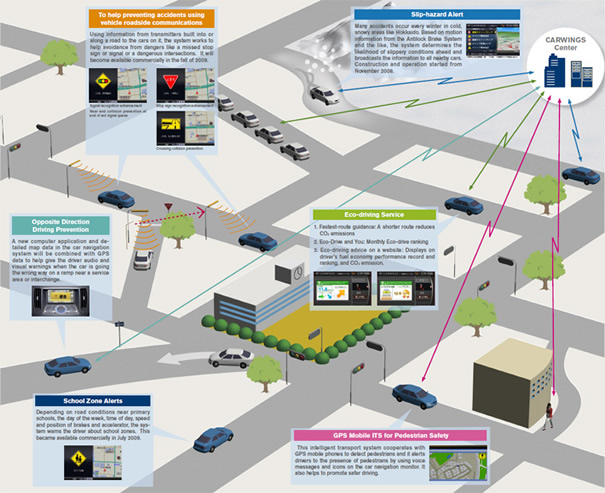
\includegraphics[scale=0.5]{Imagenes/cits}
		\caption[Ejemplo de algunos C-ITS]{Ejemplo de algunos C-ITS \protect\footnotemark}
		\label{fig:cits}
	\end{center}
\end{wrapfigure}
\footnotetext{https://www.nissan-global.com/EN/TECHNOLOGY/OVERVIEW/its.html}


Los sistemas inteligentes de transporte cooperativos, C-ITS (del inglés, \textit{Cooperative Intelligent Transport Systems}) (Figura \ref{fig:cits}), se definen como aquellos sistemas de seguridad, eficiencia y comodidad en el entorno vial, basados en el intercambio de información entre vehículos y/o insfrasestructura mediante comunicaciones inalámbricas. Incluso se puede extender al intercambio de información a usuarios que no están en el interior de un vehículo, es decir, el vehículo se encuentra conectado a un entorno cooperativo, lo que posibilita que además de poseer datos propios pueda obtener datos de su entorno.\\

\par  En pro de los avances en este área el 30 de noviembre del 2016 el Unión Europea adoptó la estrategia europea en C-ITS \footnote{https://ec.europa.eu/transport/themes/its/ } , iniciativa que tiene como objetivo facilitar la convergencia entre las inversiones y los marcos de trabajo en toda la EU, con la finalidad de poder ver estos sistemas para el 2019. En el mismo se pretende que en el 2018, se aseguren todos los aspectos legales para porporcionar certeza a los inversores públicos y privados, así como a distintos entes internacionales. Esta iniciativa consta de tres fases, siendo la primera (2014-2016), el acondicionamiento de las infraestructuras en las vías y prueba de las DSRC, la segunda (2016-2017), las primeras pruebas tangibles de estos sistemas en la sociedad y la tercera (2017-2019), la implementación definitiva de los mismos.\\

\par A través de los C-ITS se pueden realizar distintas maniobras cooperativas que pueden facilitar el trabajo en situaciones complejas, además de ayudar al conductor cuando el mismo no se encuentre en condiciones de poder reaccionar correctamente.           


\subsection{Maniobras Cooperativas}


Las investigaciones llevadas a cabo para el control de vehículos autónomos en maniobras cooperativas están en la vanguardia de los ITS. Ejemplos de estas son: maniobras de intersecciones, ACC, adelantamientos, platoonig, entre otras, descritas a continuación:

\subsubsection{ACC}

Permite fijar una velocidad de conducción y mantenerla de forma automática sin necesidad de la intervención del conductor, manteniendo una distancia de seguridad con el carro de adelante. Para poder calcular esta distancia se pueden emplear distintos dispositivos, como lo pueden ser radares, telémetros láser, o comunicaciones V2V, donde los vehículos transmiten su velocidad y posición  al resto de los vehículos \cite{van2006impact}. Cuando se emplean las comunicaiones V2V el ACC pasa a ser llamado control de crusero adaptativo cooperativo, CACC (del inglés, \textit{Cooperative Adaptative Cruise Control}) (Figura \ref{fig:acc2}) .\\  

\begin{figure}[!h]
	\centering
		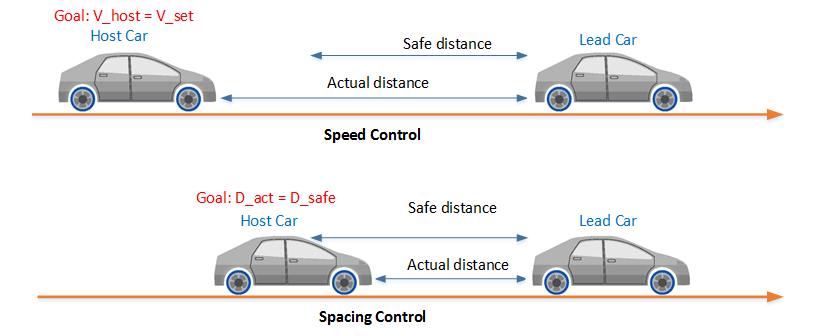
\includegraphics[scale=0.7]{Imagenes/acc2}
		\caption[Ejemplo de un CACC]{Ejemplo de un CACC \protect\footnotemark}
		\label{fig:acc2}
	\end{figure}	

\footnotetext{https://cecas.clemson.edu/cvel/auto/systems/DSRC.html}

\subsubsection{Stop And Go}

Permite acelerar y desacelerar los vehículos, cuando sea necesario, aumentando así el confort al manejar, seguridad del conductor y reducir los riesgos de colisiones. Para cumplir estos objetivos el vehículo toma acción sobre el acelerador y freno, por lo general en situaciones en el que el carro que está al frente realiza un frenado de emergencia o en momentos que se presente tráfico en la vía. Existen distintos métodos de predicción para saber cuando se debe frenar y cuando se debe acelerar, siendo las comunicaciones V2V, el método más efectivo, donde a través de la velocidad y posición del vehículo delantero se puede establecer un criterio de cuándo realizar estas acciones \cite{marzbanrad2015prediction}. En la figura \ref{fig:stg} se pueden apreciar los dos casos, cuando se frena (a) y cuando acelera (b).\\

\begin{figure}[!h]
	\centering
		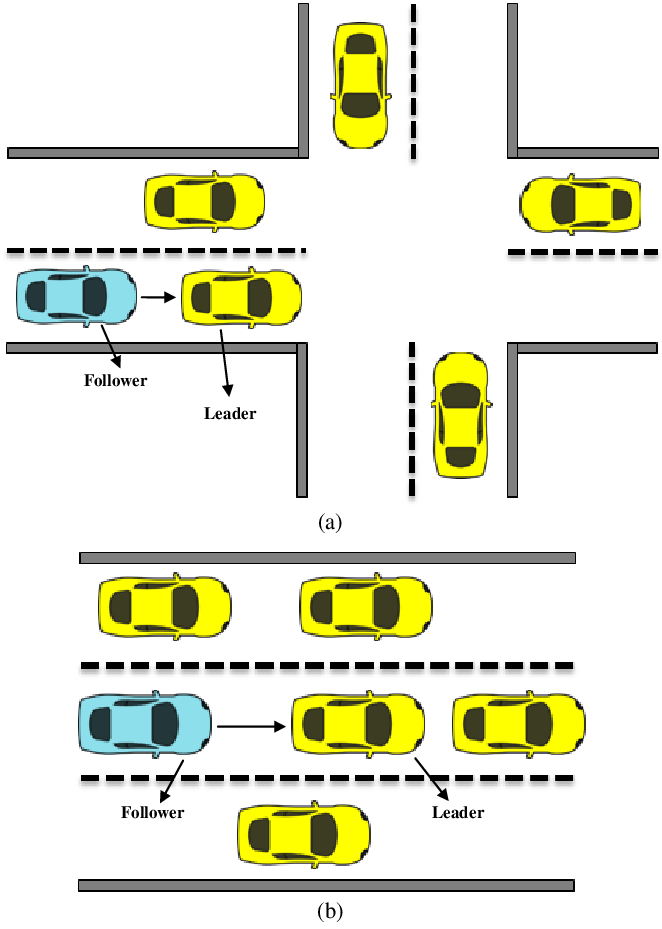
\includegraphics[scale=0.8]{Imagenes/stg}
		\caption{Ejemplo de un Stop and Go \cite{marzbanrad2015prediction}}
		\label{fig:stg}
	\end{figure}	

 
\subsubsection{Control Lateral}

Permite controlar el volante dependiendo de la posición del vehículo delantero, es decir controla el moviento lateral, tomando en cuenta las acciones del carro que tenga adelante, y de esta forma realizar la conducción del vehículo que permita al conductor descansar en momentos de mucho cansancio. Para lograr esta forma de conducción se emplean las comunicaciones V2V, en donde el vehículo delantero transmite su posición y dirección, para que el carro seguidor ajuste su posición con respecto a esta. En la figura \ref{fig:cl} se puede ver un ejemplo del control lateral en un cambio de canal.\\


\begin{figure}[!h]
	\centering
		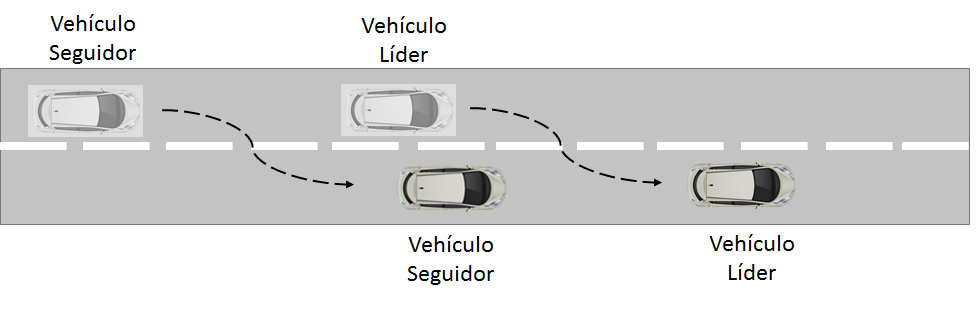
\includegraphics[scale=0.6]{Imagenes/cl}
		\caption{Ejemplo de un Contol Lateral}
		\label{fig:cl}
	\end{figure}	

 

\subsubsection{Platoonig}

Permite que un grupo de vehículos puedan viajar a una distancia segura, y a altas velocidades. En esta maniobra el carro líder fija la velocidad y dirección del grupo, enviándo mediante comunicación V2V, su velocidad, posición y dirección a los demás integrantes del grupo, para que los mismos se ajusten tomando como referencia estos datos. Con esta forma de conducción se reducen los riesgos de colisiones, así como una optimización de la cantidad de vehículos en las autopistas. En la Figura \ref{fig:plat} se puede apreciar un ejemplo de Platooning, donde el vehículo líder es un camión que guía a los demas carros.\\

\begin{figure}[!h]
	\centering
		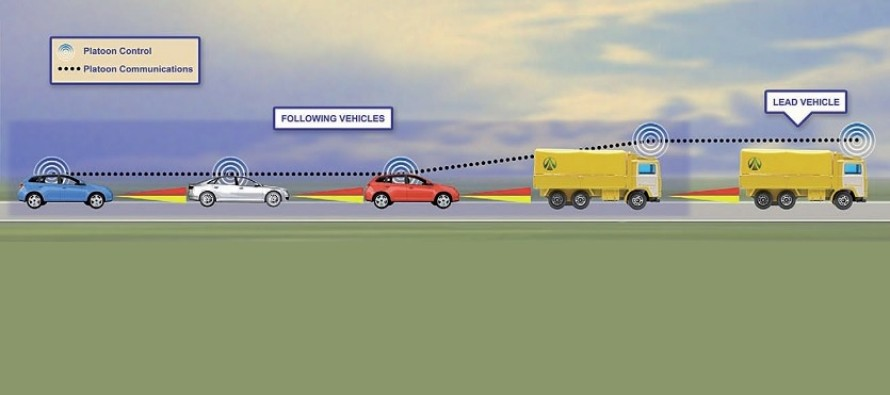
\includegraphics[scale=0.6]{Imagenes/plat}
		\caption[Ejemplo de un Platooning]{Ejemplo de un Platooning \protect\footnotemark}
		\label{fig:plat}
	\end{figure}	

 \footnotetext{http://www.driverlesstransportation.com/platooning-1157}


\section{Lógica Borrosa}

La lógica borrosa se puede definir como una lógica multivaluada que permite representar matemáticamente la incertidumbre y la impresición, proporcionando herramientas formales para su tratamiento. Básicamente, cualquier problema del mundo se puede resolver a través de un conjunto de variables de entradas, las cuales proporcionan un valor adecuado de variables de salidas. El término fue acuñado por primera vez en 1974 por Lofti A. Zadeh, donde la presentó como una forma de procesamiento de información en la que los datos podrían tener asociados un grado de pertenencia parcial a conjuntos. Además describió el concepto de conjunto difuso y su función de pertenencia asociada, la cual toma valores en el intervalo unitario, y siendo en la década de los 90 que se introdujeron los conceptos restantes, variable linguistica y de reglas if-then \cite{morcillo2011logica}.\\

\par Para que la lógica borrosa pueda lograr su objetivo, se establecen conjuntos difusos que proporcionan la imprecisión de forma cuantitativa al cual será sometido el valor. Dichos conjuntos se manifiestan a través de funciones de membresía o pertenencia las cuales entregan el grado de pertenencia de un valor hacia un tributo establecido.\\

\par Para ejemplificar mejor estos conceptos, se procederá a describir el caso de la altura en los hombres. Según la lógica clásica se definen dos conjuntos, hombres altos y hombres bajos, quienes se constituyen de hombres mayor a 1.8 m y menor a dicho valor, es decir cualquier hombre cuya estatura sea 1.79 m será considerado como bajo, y uno de 1.81 m, como alto. En la lógica difusa no solo se tienen dos conjuntos estrictamente definidos, si no que se tienen conjutos intermedios, los cuales permiten una transición entre un caso y el otro, es decir un hombre puede tener una estatura de 1.78 m con un grado de certeza de 0.8 y bajo con un grado de certeza de 0.2, mientras que en el caso de un hombre de 1.60 m de estatura, este puede pertenecer al conjunto de hombres bajos con 0.9 grados y al de hombres altos con 0.1 grados. Dicha comparación puede ser mejor apreciada en la figura \ref{fig:hombres}.\\

\begin{figure}[!h]
	\centering
		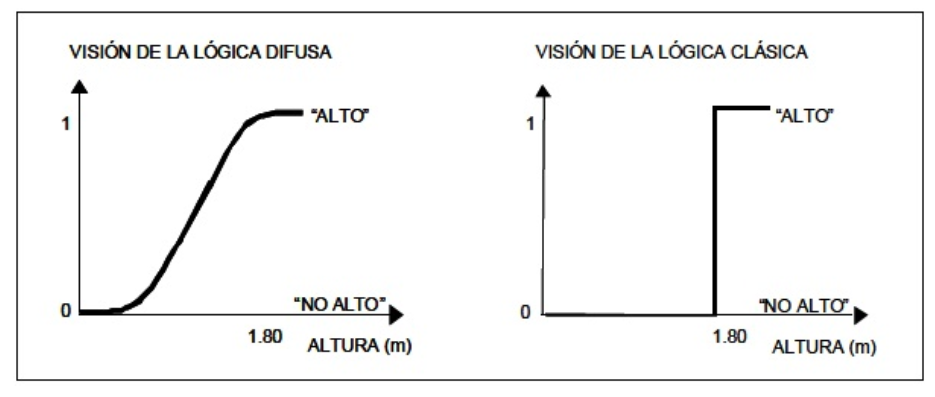
\includegraphics[scale=0.7]{Imagenes/hombres}
		\caption{Lógica clásica vs Lógica difusa \cite{fuzzy}}
		\label{fig:hombres}
	\end{figure}	

\subsection{Control Borroso}

Los controladores borrosos surgen en los años 60, como una herramienta empleada en el control de procesos complejos de cualquier tipo, permitiendo dar valores intermedios entre dos extremos a una variables que se desea manipular, y con esto hacer posible que la lógica humana sea empleada de manera directa.\\

\par Estos controladores reciben entradas analógicas debido a su rango no discreto y se clasifican por el grado de membresía de sus conjuntos, los cuales corresponden a reglas implementadas que aplican la lógica humana para determinar de que forma los conjuntos difusos o sus combinaciones, definen la(s) salida(s) del controlador. En la figura \ref{fig:fuzzy} se puede encontrar un esquema de la representación de estos controladores.\\ 

\begin{figure}[H]
	\centering
		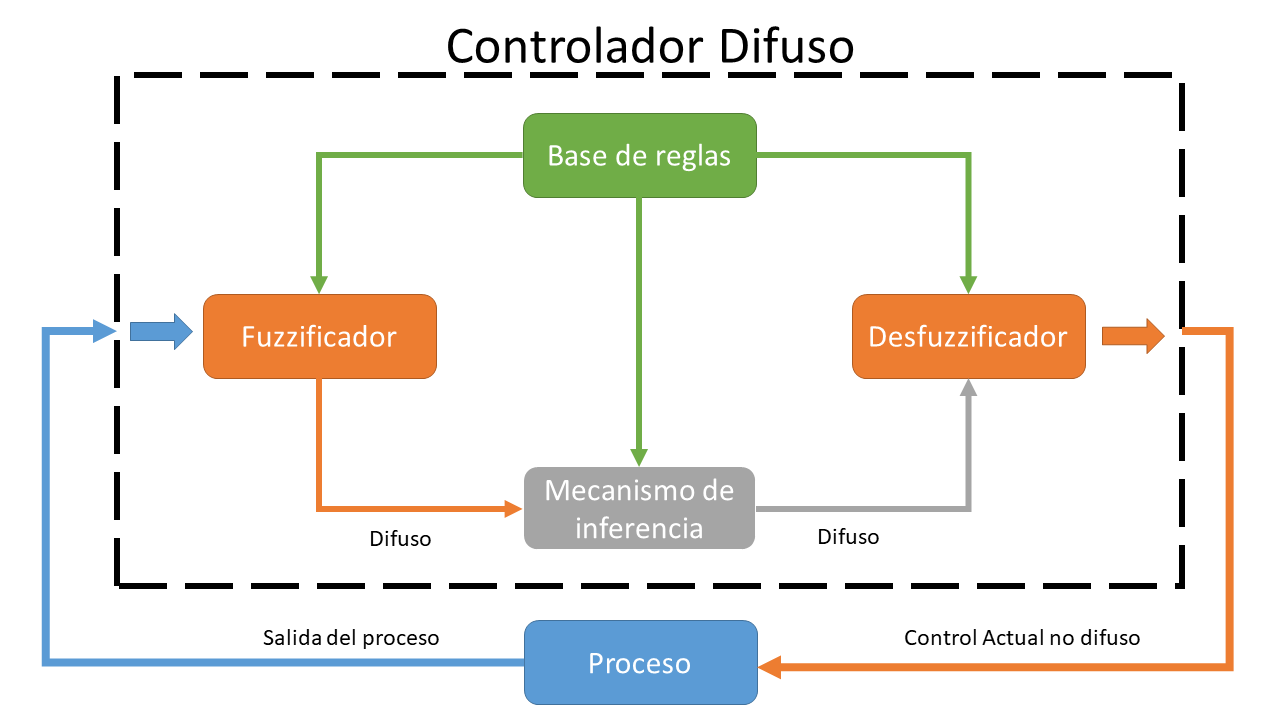
\includegraphics[scale=0.5]{Imagenes/fuzzy}
		\caption{Esquema de un controlador borroso}
		\label{fig:fuzzy}
	\end{figure}	

\par Como se puede apreciar los controladores borrosos están compuestos por varias etapas, los cuales consisten en \cite{fuzzy}:

\begin{itemize}
	\item Fuzzyficación: Esta estapa consiste en transformar la(s) variable(s) de entrada en un grado de pertenencia que cuantifica el grado de membresía de los determindos conjuntos difusos. Es en este proceso donde las funciones de membresía son aplicadas, más comunmente tienen foma de trapezoides, triángulos, gaussianas, etc. Definiendo de esta forma el grado de transición de pertenencia entre un conjunto y otro, permitiendo así, que la etapa de inferencia pueda interpretar la entrada de forma correcta 
	\item Inferencia: Es en esta etapa que se representa verdaderamente la lógica del controlador, es donde se evaluan las entradas "fuzzyficadas" de la etapa anterior, a través de condiciones definidas,  las cuales permiten calcular la salida del mismo. La base de reglas está constituida por una serie de condiciones que consideran la(s) entrada(s) y establecen cuantitativamente salidas difusas que posteriormente serán interpretadas por la etapa final. Dentro de esta fase se pueden encontrar dos métodos importantes, Mamdani y Takagi-Sugeno, que consisten en \cite{jang1996input}:
	\subitem Mamdani: es posiblemente el método más empleado, propuesto por Ebrahim Mamdani en 1975, este método busca obtener un único número que represente el resultado, a través de la evaluación de los grados de pertenencia en las reglas propuestas. En el caso de de que una regla tenga multiples antecedentes se utilizan los operadores AND u OR, dependiendo de lo que se busque, en el caso del operador AND se suele usar la T-Norma estándar del mínimo y para el OR la T-Conorma estándar del máximo. Finalmente con el resultado de esta evaluación se aplica un recorte o escalado a las funciones de salida para unificarlas, y así obtener el valor.
	\subitem Takagi-Sugeno: este método emplea los mismos principios que Mamdani, con la única diferencia que, para obtener el valor de salida no se emplean funciones de pertenencia, sino que se asignan valores númericos a las reglas, reduciendo el coste computacional con respecto a mandani, pero perdiendo la representación del conocimiento humano.     
	\item Desfuzzycación: Es la última etapa que realiza el controlador, es donde se estalece(n) la(s) salida(s) del mismo, a partir de las reglas evaluadas en la etapa procedente. Dependiendo del método de inferencia empleado se pueden utilizar técnicas como el centro de gravedad o centro promediados para el caso de Mamdani, o funciones ponderadas para el caso de Takagi-Sugeno.    
\end{itemize}


\section{Resumen}

En el presente capítulo se presenta el estado del arte, donde primero se resumieron algunos puntos de importancia para entender, cómo están estructurados los sistemas de comunicaciones actualmente, como lo son el modelo de capas OSI y las redes ad-hoc, así como tambien los protocolos de transporte que se emplean hoy en día.\\

\par De igual forma se presentó una descripción extensa de los protocolos de comunicación, tanto vehiculares, como comerciales. Donde también se explicó el cómo surgió cada uno, sus componentes y sus usos.\\

\par Finalmente se mencionaron los C-ITS y de cómo estos pueden ayudar con distintos problemas que se presentan a la hora de conducir. Para luego dar a conocer algunas maniobras que se pueden realizar con estos sistemas, más específicamente las que se realizaron en este trabajo, y para cerrar se describieron los fundamentos sobre los cuales estan basados los controladores borrosos, controladores empleados para el desarrollo de las maniobras cooperativas presentadas.      






